%%%%%%%%%%%%%%%%%%%%%%%%%%%%%%%%%%%%%%%%%%%%%%%%%%%%%%%%%%%%%%%%%%%%
%%%%%%%%%%%%%%%%%%%%%%%%%%%%%%%%%%%%%%%%%%%%%%%%%%%%%%%%%%%%%%%%%%%%
\chapter{Reference}

% ==================================================================
\section{Overview}

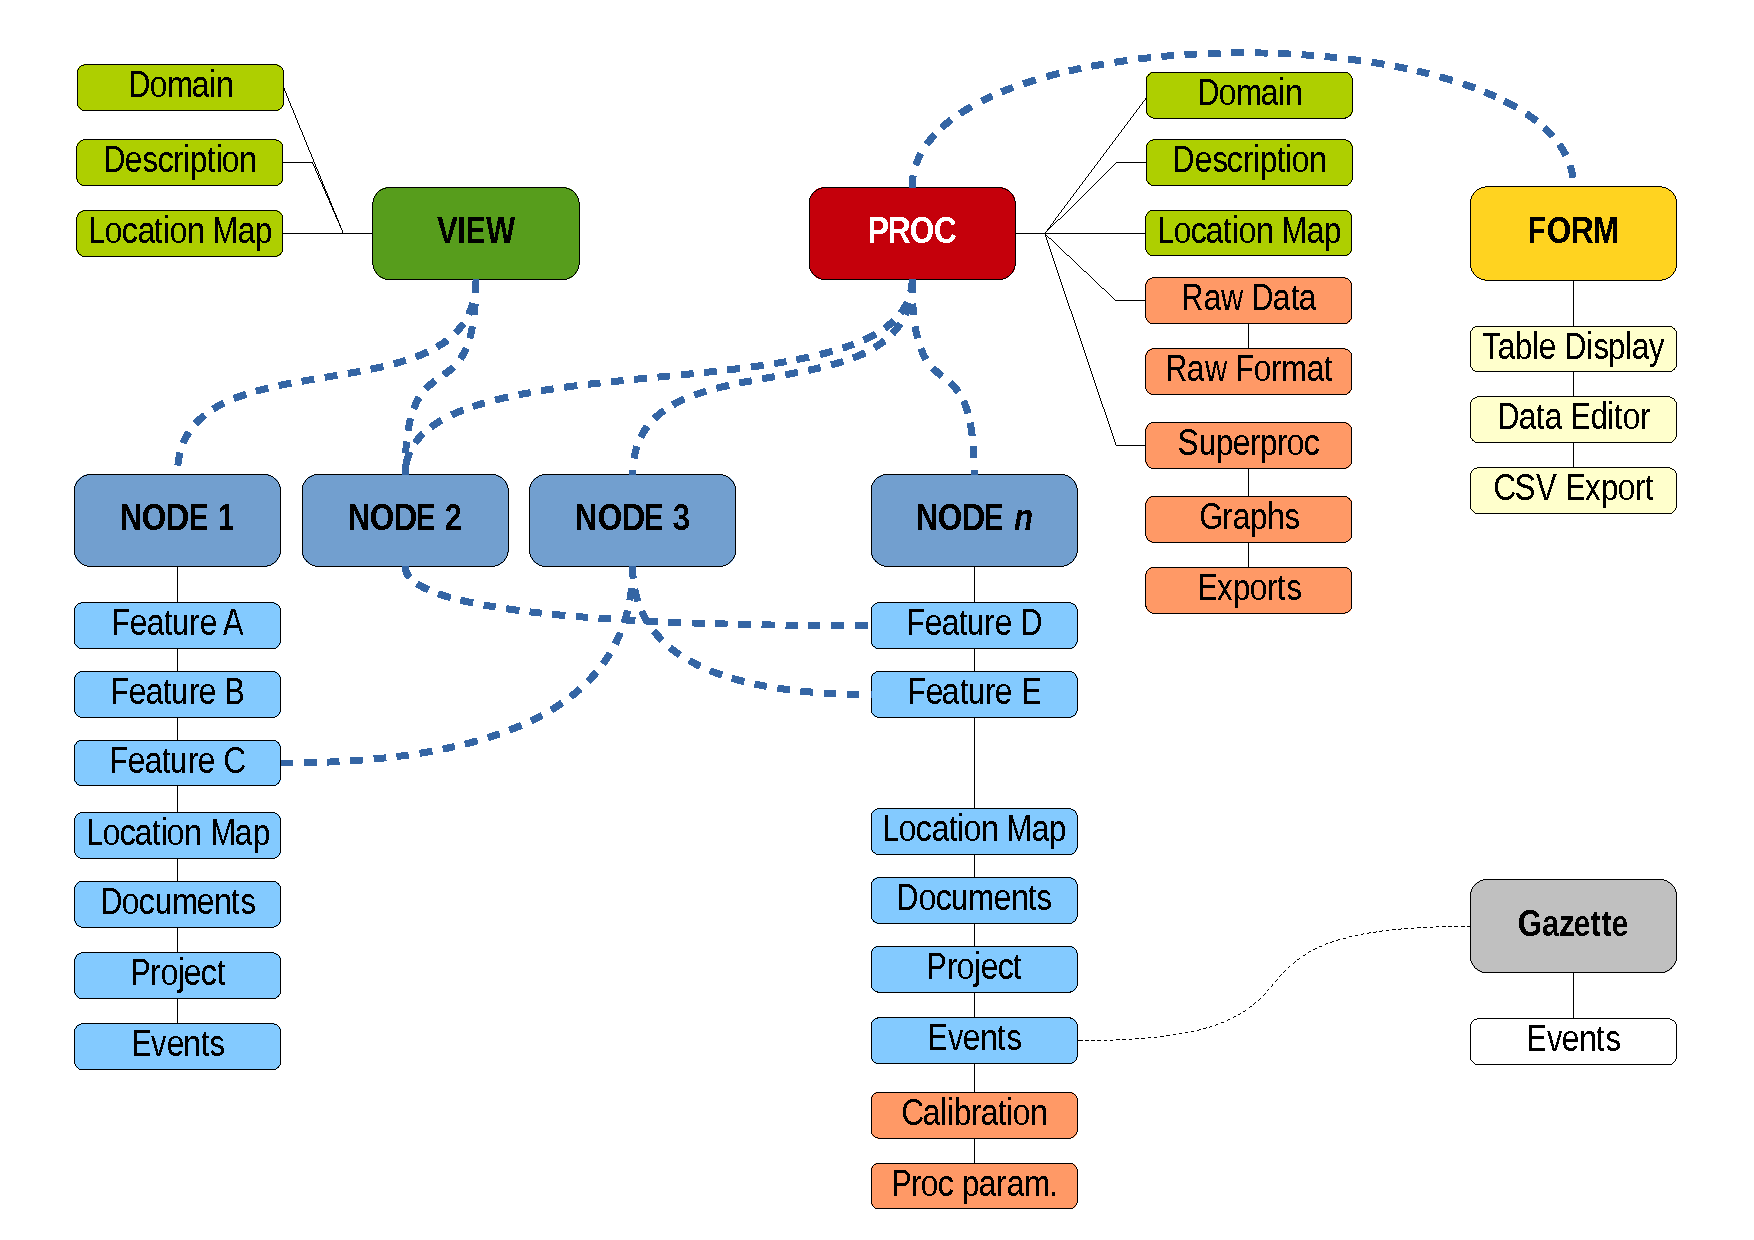
\includegraphics[width=\textwidth]{figures/webobs_diagram.pdf}

% ==================================================================
\section{Nodes: Elementary WebObs Objects}

A \wo{node} is the central \webobs element associated with following attributes:

\begin{itemize}
\item    a long name (\wo{name}) and short name (\wo{alias});
\item    an optional short description (\wo{type});
\item    a lifetime period with start and end dates (both optional);
\item    a time zone (associated to lifetime dates and events date/time);
\item    an optional location (latitude, longitude, elevation) associated with a location map (graph), OpenStreetMap GUI and KML link;
\item    optional text contents for "informations", "installation" and "access";
\item    an optional sensor description associated with a calibration table of channels parameters;
\item    a list of user-defined features (also free text contents);
\item    attached documents, photos and diagrams;
\item    a project;
\item    events log associated with date and operator list;
\item    a list of associated grids (\wo{views} and/or \wo{procs}, see \ref{grids});
\item    a validity flag (for admin users);
\item	 optional functional parameters when the \wo{node} is associated to a \wo{proc}: data code (\wo{FID}), network code (\wo{FDSN}), data format (\wo{RAWFORMAT}) and source (\wo{RAWDATA}), time zone (\wo{TZ}) of data, acquisition period and delay, and a calibration file that describes each channel characteristics and history:
	\begin{itemize}
	\item    date and time of validity;
	\item    channel number, name, unit, code, S/N, offset, factor, gain, min/max values, azimuth, latitude, longitude, elevation, depth, sampling frequency, dynamic, location code.
	\end{itemize}
\end{itemize}

Examples of what a \wo{node} can be:
\begin{itemize}
\item    an instrumental station or a part of it,
\item    a site or place for data sampling or measurement,
\item    a place of any interest,
\item    a mobile equipment, an instrument, a building, a vehicle, ...
\item    a journal board, an event description (e.g. an historical earthquake), ...
\end{itemize}


\lstinputlisting[title=\wofile{NODES.rc}]{../../SETUP/CONF/NODES.rc}

% -----------------------------------------------------------------
\subsection{Create, edit or delete a NODE}

Modifying \wo{node} is possible only through a \wo{grid} (see next section \ref{grids}). Creation of new \wo{node} or edition of an existing \wo{node} deserves to \wo{users} with edit level for the associated \wo{grid}. Deletion of a \wo{node} is reserved to administrator level \wo{users}.

% -----------------------------------------------------------------
\subsubsection{Node validity}

Once created, a \wo{node} can be valid or invalid. When invalid, a \wo{node} exists but is hidden for standard \wo{users}. It will be ignored by most of the \webobs processes (like \wo{procs}). Nevertheless, if a \wo{user} has an administrator level, he will be able to see an invalid \wo{node} in the lists and tables, and make it valid if necessary.


% -----------------------------------------------------------------
\subsection{Names and codes}

% - - - - - - - - - - - - - - - - - - - - - - - - - - - - - - - - -
\subsubsection{Main code (ID)}

Each \wo{node} has a unique ID code in \webobs. The code can be any string of characters, but it is recommended to use a comprehensive and rational code (see appendix \ref{nodeidcodes}) when creating a new \wo{node}. Attribution of this unique code deserves to \wo{users} with administrator level when creating a new \wo{node}. It cannot be modified after.


% - - - - - - - - - - - - - - - - - - - - - - - - - - - - - - - - -
\subsubsection{Name}

The long NAME of a \wo{node} is used for display purposes in tables and graphs. It cannot be empty. The NAME is displayed in the main GRID's table in front of the corresponding \wo{node}.


% - - - - - - - - - - - - - - - - - - - - - - - - - - - - - - - - -
\subsubsection{Alias (short name)}

The ALIAS is the short name of a \wo{node}, used for display purposes in table and graphs. It cannot be empty. The ALIAS is displayed in the main GRID's table in front of the corresponding \wo{node}.



% - - - - - - - - - - - - - - - - - - - - - - - - - - - - - - - - -
\subsubsection{Type}

The TYPE of a \wo{node} is an optional free string that will be used for any short description of the \wo{node}. The TYPE is displayed in the main GRID's table in front of the corresponding \wo{node}.


% -----------------------------------------------------------------
\subsection{Lifetime and time zone}

% - - - - - - - - - - - - - - - - - - - - - - - - - - - - - - - - -
\subsubsection{Start/end dates}

Start and end dates of a \wo{node} define the period of activity of this \wo{node}. Both or any of these two dates can be undefined or incompletely defined, while respecting the ISO 8601 standard: Date values are ordered from the most to the least significant: year, month and day; any number of values may be dropped from any of the date representations, but in the order from the least to the most significant. For example, 1976 and 2005-04 are both reduced precision valid dates.

The lifetime of a \wo{node} has potential impact on processes that use this \wo{node} or associated data.


% - - - - - - - - - - - - - - - - - - - - - - - - - - - - - - - - -
\subsubsection{Time zone}

A time zone (in hours relative to GMT, in the format \wokey{+/-HH[MM]}) is used to define the lifetime and dated events (see below).

% -----------------------------------------------------------------
\subsection{Grids memberships}

A \wo{node} can be associated with one or more \wo{grids}. See section \ref{grids}.

% -----------------------------------------------------------------
\subsection{Geographic location}

\includegraphics[width=\textwidth]{figures/NODE_location.png}

A \wo{node} can be georeferenced using latitude, longitude and elevation coordinates on Earth. When a \wo{node} has valid coordinates defined, a location map will be automatically built (see below and section \ref{locastat}), and it will appear on associated GRID's maps (see section \ref{grids}).

% - - - - - - - - - - - - - - - - - - - - - - - - - - - - - - - - -
\subsubsection{WGS84 coordinates}

Latitude and longitude must be in the WGS84 geodetic reference system, and expressed in decimal form, using negative value for southern latitude and western longitude. Use the dot as decimal point (not coma).

In the \wo{node}'s display page, coordinates are presented in different formats: DDD.ddddd (decimal degrees), DDD\degree MM.mmm' (degrees and decimal minutes) and DDD\degree MM'SS.s" (degrees, minutes and decimal secondes).

The coordinates are displayed in the main GRID's table in front of the corresponding \wo{node}. Also, the Universal Transverse Mercator (UTM) projection is computed and displayed in the \wo{node}'s page.

% - - - - - - - - - - - - - - - - - - - - - - - - - - - - - - - - -
\subsubsection{Timestamp and type of coordinates}

This optional information provides the timestamp (date) of coordinates, and a type of positioning from a list.

\lstinputlisting[title=\wofile{POSITIONtypes.conf}]{../../SETUP/CONF/POSITIONtypes.conf}


% - - - - - - - - - - - - - - - - - - - - - - - - - - - - - - - - -
\subsubsection{OpenStreetMap API link}

Link to OpenStreetMap API is available if the \wo{node} has coordinates. The link will open a pop-up window. This functionality is associated with some variables in the main configuration file \wofile{WEBOBS.rc}:

\begin{lstlisting}[title=\wofile{WEBOBS.rc} (excerpt)]
CGI_OSM|OSM.pl
OSM_LINK|1
OSM_INFO|See with OpenStreetMap
OSM_NODE_ICON|/icons/gdot.png
OSM_WIDTH_VALUE|800
OSM_HEIGHT_VALUE|600
OSM_ZOOM_VALUE|17
\end{lstlisting}

% - - - - - - - - - - - - - - - - - - - - - - - - - - - - - - - - -
\subsubsection{KML link}

Link to a KML file is available if the \wo{node} has coordinates. The link will download a local KML file, which may be open with local application associated with KML file type (e.g., Google Earth). This functionality is associated with some variables in the main configuration file \wofile{WEBOBS.rc}:

\begin{lstlisting}[title=\wofile{WEBOBS.rc} (excerpt)]
GOOGLE_EARTH_LINK|1
GOOGLE_EARTH_LINK_INFO|KML file for Google Earth (ATTENTION: error ~20 m)
IMAGE_LOGO_GOOGLE_EARTH|/icons/google/google_earth.gif
\end{lstlisting}

% - - - - - - - - - - - - - - - - - - - - - - - - - - - - - - - - -
\subsubsection{Location map}

A location map with 4 different scales is automatically made and updated by LOCASTAT application (see section \ref{locastat} for associated parameters), using the coordinates of the \wo{node}.


% - - - - - - - - - - - - - - - - - - - - - - - - - - - - - - - - -
\subsubsection{Neighbour nodes}

A list of neighbour nodes is automatically displayed, sorted by decreasing distances and indicating direction and elevation gain relative to the displayed node. A link to each neighbour nodes is available, with a warning icon when a project is associated to this node. 

% -----------------------------------------------------------------
\subsection{Transmission}

When a \wo{node} represents, for instance, an instrumental station with data transmission, the type of transmission can defined using a reference list (below) and other \wo{node}s can be defined as intermediate repeaters or final acquisition point.

The transmission chain is displayed with dynamic links to associated \wo{node}s. It appears also on the location map (see section \ref{locastat}) and the \wo{grid} maps (see section \ref{gridmaps}).

% - - - - - - - - - - - - - - - - - - - - - - - - - - - - - - - - -
\subsubsection{Type}

Type of transmission is defined in a list of transmission type associated with plot line style, width and color.

\lstinputlisting[title=\wofile{TRANStypes.conf}]{../../SETUP/CONF/TRANStypes.conf}


% - - - - - - - - - - - - - - - - - - - - - - - - - - - - - - - - -
\subsubsection{Acquisition and repeaters}

The transmission chain is described by defining a list of \wo{node}'s ID, from station to acquisition.


% -----------------------------------------------------------------
\subsection{Features}

Each \wo{node} can have user-defined features which are free text contents (HTML and Wiki syntax allowed) that appear in the main table as a series of table cells.

% - - - - - - - - - - - - - - - - - - - - - - - - - - - - - - - - -
\subsubsection{List of user-defined features}

Feature name is limited to short names and must avoid special characters. Edit the list of features to be displayed using the \wo{node} configuration form. Features with void content won't be displayed for \wo{users} without edit or admin rights.

% - - - - - - - - - - - - - - - - - - - - - - - - - - - - - - - - -
\subsubsection{Node-features-nodes association list}

It is possible to associate a \wo{node}'s feature to an other \wo{node} as its feature's children. An automatic link will be displayed in the feature's table cell before the text content of the feature. In the children \wo{node} page, the parent feature will appear with automatic name "feature of" and a link to the parent \wo{node}.

For administrators, the node2node association list is stored in a single configuration file containing a 3-field definition (pipe delimited):

\begin{lstlisting}[title=\wofile{nodes2nodes.rc} (excerpt)]
PARENT_NODEID|featurename|CHILDREN_NODEID
\end{lstlisting}


% -----------------------------------------------------------------
\subsection{Proc's parameters and data status}
\label{nodeprocparam}
When associated with a \wo{proc} (see section \ref{procs}), data from a \wo{node} is used to produce outputs. Several additional parameters must be defined for this.


% - - - - - - - - - - - - - - - - - - - - - - - - - - - - - - - - -
\subsubsection{Network code}

A \wo{node} can be associated with a standard network code, from the International Federation of Digital Seismograph Networks (FDSN)~\footnote{see \url{http://www.fdsn.org/}}. This is mostly the case for permanent seismological stations. This code is mandatory when using Arclink or Seedlink data requests (see sections \ref{seedlink} and \ref{arclink}).

The list of network codes is also described at IRIS~\footnote{see \url{http://www.iris.edu/ds/nodes/dmc/services/network-codes/}}.

The official FDSN codes list can be overwritten using a local configuration file \wofile{CONF/networkcodes.csv}.

% - - - - - - - - - - - - - - - - - - - - - - - - - - - - - - - - -
\subsubsection{Raw format}

A list of possible data format that overwrites, if selected, the \texttt{RAWFORMAT} parameter in the PROC/*.conf. This allows to associate different data format/source to the NODEs associated to a single PROC.


% - - - - - - - - - - - - - - - - - - - - - - - - - - - - - - - - -
\subsubsection{Raw data source}

A free text string that overwrites, if not blank, the \texttt{RAWDATA} parameter in the PROC/*.conf. This allows to associate different data format/source to the NODEs associated to a single PROC.


% - - - - - - - - - - - - - - - - - - - - - - - - - - - - - - - - -
\subsubsection{FID}

A FID code is a short string which may contain a functional code (or a coma-separated list of codes) that will be used by associated PROCs. For example, it can be the official station code for a seismic station or a GNSS receiver, while the data files will contain this code. It is generally set to the same string as the ALIAS.

Some \wo{procs} are able to deal with a coma-separated list, as gnss: this allows to define multiple codes pointing to different data, and associate them to a single station.

% - - - - - - - - - - - - - - - - - - - - - - - - - - - - - - - - -
\subsubsection{FID\_*}

Some raw formats may need additional codes or parameters to process data from the \wo{node}. It is possible to define specific parameters with the prefix \wo{FID\_}: they will be listed and editable below the main FID. Creation/edit of a \wo{FID\_SUBNAME} is reserved to \wo{users} with administrator level.


% - - - - - - - - - - - - - - - - - - - - - - - - - - - - - - - - -
\subsubsection{Time zone}

Time zone is the offset delay from UTC, expressed in hours. Examples: $+0$ is UTC, $-4$ is Lesser Antilles time.

% - - - - - - - - - - - - - - - - - - - - - - - - - - - - - - - - -
\subsubsection{Acquisition period}

Acquisition period defines the normal time interval between two data sample, expressed in days. Examples: \texttt{1/24} corresponds to 1 sample per hour, \texttt{1/86400} is 1 Hz sampling. This value might be used to compute average acquisition performance rating (see below).

% - - - - - - - - - - - - - - - - - - - - - - - - - - - - - - - - -
\subsubsection{Acquisition delay}

This value defines the maximum delay allowed between the last available data and the present time, expressed in days. This delay is used to determine the \wo{node}'s status (see below).

% - - - - - - - - - - - - - - - - - - - - - - - - - - - - - - - - -
\subsubsection{Status and link to data}

If the associated \wo{proc} is set to compute the \wo{node} status, the following information is displayed:
\begin{itemize}
\item last status check timestamp;
\item sampling rate performance (in \%): number of valid samples over the last time period, compared to theoretical acquisition period (see above);
\item status (in \%): existence of valid samples in the last time delay for all channels.
\end{itemize}

The status informations are displayed in the main GRID's table in front of the corresponding \wo{node}.

If the associated \wo{proc} produces output graphs, direct links to each outputs are available.


% - - - - - - - - - - - - - - - - - - - - - - - - - - - - - - - - -
\subsubsection{Channels parameters (calibration file)}
\label{clb}

\includegraphics[width=\textwidth]{figures/CLB_table.png}

For most of \wo{procs}, it is mandatory to define a list of data channels. This can be done through a ``calibration file'' that contains description and detailed parameters of the \wo{node}'s data channels: date and time of validity, name, unit, S/N, functional code, gain and multiplier factors, offset, min/max values, sensor azimuth, location and depth, sampling frequency, digital dynamic and ``location code'' (SEED standard). Each channel must have one or more series of parameters. 

The date and time of validity applies until real-time or next line of parameters for this channel number.

Each \wo{proc} might be associated to a selection of channels. Active channels appear in bold font, while inactive appear in gray.


% -----------------------------------------------------------------
\subsection{Installation, information and access}

These 3 fields are free-length text content. Wiki syntax allowed.

% -----------------------------------------------------------------
\subsection{Photos, diagrams and associated documents}

Three different types of documents can be uploaded and associated to a \wo{node}:
\begin{itemize}
	\item Photos: any JPEG file that will be displayed as thumbnail with a link to full screen mode;
	\item Diagrams: any image or picture file (JPEG, GIF, PNG, PDF, ...) that will be displayed as thumbnail with a link to the full resolution image;
	\item Documents: any file (PDF, DOC, TXT, ...) that will be downloadable and sometimes displayed through the navigator.
\end{itemize}


% -----------------------------------------------------------------
\subsection{Project}
\label{projectnode}

A \wo{node} may have one (and only one) \wo{Project} description: a free-length text file, accepting MultiMarkDown syntax, a list of users and possible associated photos. Project is a special \wo{Event} without date.

% -----------------------------------------------------------------
\subsection{Events}
\label{eventnode}

A \wo{node} can be associated to dated events. A \wo{node} event has following characteristics:
\begin{itemize}
	\item start date and time;
	\item end date \& time;
	\item a title;
	\item a content of free-length text,
	\item author(s) from the list of \webobs users;
	\item selected feature (from the node's feature list);
	\item sensor/data outcome flag;
	\item notebook number (optional);
	\item notebook forward flag (optional);
	\item associated photos (image files).
\end{itemize}
An event can include one or more sub-events (children). Event files  accept the MultiMarkDown syntax. See \wo{Events logging} section (\ref{events:logging}) for a description of Nodes and Grids events coding.


% ==================================================================
\section{Grids: networks of nodes}
\label{grids}

A \wo{grid} is a group of \wo{nodes}. Each \wo{node} can be associated to one or multiple \wo{grids}. There is two kind of \wo{grids}:

\begin{itemize}
\item    A \wo{view} is a list of \wo{nodes} we simply want to group to be seen or accessed together,
\item    A \wo{proc} is a list of \wo{nodes} associated to a common data processing that produces outputs (graphs and/or elaborated data), and/or optional editable data FORMS.
\end{itemize}

\wo{grids} are presented through a sorted table allowing access to dedicated page for each \wo{grid} with:
\begin{itemize}
\item    domain: a category used to group similar \wo{grids};
\item    purpose (text content);
\item    specifications: operator owner, number of \wo{nodes}, type, optional external link;
\item    list of \wo{nodes}: a complete table with alias, names, location, start/end dates, type, project, status (for active \wo{proc}); ...
\item    an interactive location map (if at least one \wo{node} is georeferenced);
\item    informations (text content);
\item    references (text content);
\item    a graphical representation of \wo{nodes} links with associated \wo{grids}.
\end{itemize}

Text content sections are editable with Wiki syntax possibilities.

%\includegraphics[width=\textwidth]{figures/PROC_GEOSCOPE_map.png}


\lstinputlisting[title=\wofile{GRIDS.rc}]{../../SETUP/CONF/GRIDS.rc}

% -----------------------------------------------------------------
\subsection{Domains}
\label{domains}

A \wo{domain} is a generic category that is used to group \wo{grids} together: in the \wo{grid}'s table presentation and in most of the page links between \wo{grids} and \wo{nodes}. By default, \wo{domains} are defined as a list of standard scientific methods as used in volcanological observatories: Seismology, Deformations, Geochemistry, Imagery, ... but these categories can be changed to better fit the \webobs needs. For example, if the \webobs has to handle multiple targets (like volcanoes), you might want to make the \wo{domains} as a list of these targets.

Changes to \wo{domains} list can be done by administrator by editing the sqlite database. New domains can be easily added by inserting an entry into the \wokey{domains} table. To remove an existing \wo{domain}, you must remove any \wo{grid} associated to this \wo{domain} first (this can be done using the GUI of \wo{grid} configuration editor), then delete manually the entry in the database. 

\begin{lstlisting}[title=\wofile{WEBOBS.rc} (excerpt)]
SQL_DOMAINS|${ROOT_CONF}/WEBOBSDOMAINS.db
SQL_TABLE_DOMAINS|domains
SQL_TABLE_GRIDS|grids2domains
\end{lstlisting}



% -----------------------------------------------------------------
\subsection{Views}
\label{views}

A \wo{view} is a simple group of NODES.

To create a new \wo{view}, go to any \wo{GRID} table page (menu GRIDS, VIEWS or PROCS) and click on the edit icon in the Name header of table, enter an unique short name and click Edit. This will open the \wo{grid} configuration editor. The form allows to freely edit the parameters file (key/value pairs), to select the Domain and to associate/disassociate \wo{nodes}.

\lstinputlisting[title=\wofile{VIEW.DEFAULT} template]{../../CODE/tplates/VIEW.DEFAULT}

All the following parameters are valid for \wo{grids}, that is any \wo{view} or \wo{proc} (see the next section).

% - - - - - - - - - - - - - - - - - - - - - - - - - - - - - - - - -
\subsubsection{\wo{grid} name and attributes}
\begin{itemize}

\item \wokey{NAME}: Character string for the \wo{grid} long name. This name will appear in the \wo{grid} page and maps of \wo{nodes}.

\item \wokey{OWNCODE}: Character string for the \wo{grid}'s owner name. This name will be displayed in the \wo{grids} tables and \wo{grid} summary, if \wokey{SHOW\_OWNER} key is true in \wofile{GRIDS.rc}. For backward compatibility, the key might contains a short code with corresponding long names in \wofile{CONF/OWNERS.conf}.

%\lstinputlisting[title=\wofile{OWNERS.conf} template]{../../SETUP/CONF/OWNERS.conf}

\item \wokey{TYPE}: Character string giving a short attribute to the \wo{grid}, if \wokey{SHOW\_TYPE} key is true in \wofile{GRIDS.rc}.

\item \wokey{URL}: Optional URL related to the \wo{grid}. Any valid URL is allowed, e.g. an external web link.

\item \wokey{COPYRIGHT}: Optional character string for the copyright of the \wo{grid}.

\end{itemize}


% - - - - - - - - - - - - - - - - - - - - - - - - - - - - - - - - -
\subsubsection{\wo{NODES} attributes}
\begin{itemize}

\item \wokey{NODE\_NAME}: Short name of a generic \wo{node}. This name will be used instead of ``node'' in tables and maps.

\item \wokey{NODE\_MARKER}: Type of marker used to plot \wo{nodes} on maps. See valid markers in table \ref{markertype}.

\item \wokey{NODE\_SIZE}: Size of the \wo{node} marker for maps (in points).

\item \wokey{NODE\_RGB}: Color of the \wo{node} marker for maps: it can be a color name string (see \wofile{CODE/matlab/htm2rgb.m} for a list of standard colors), or a vector of 3 scalars (red,green,blue), each value between 0 and 1.

\item \wokey{NODE\_FONTSIZE}: If not empty, font size to display \wo{node}'s alias names on maps besides the marker. A

\end{itemize}



% -----------------------------------------------------------------
\subsection{Procs}
\label{procs}

A \wo{proc} is a list of \wo{nodes} that are associated to a specific and common data processing called \wo{superproc}. It has the same basic parameters as \wo{views} (see previous section \ref{views}) plus additional settings that depend on the process you want to achieve. \webobs proposes some built-in \wo{superprocs} (see chapter \ref{builtin}), each of them are specific. There is on default \wo{superproc} called 'genplot' which is a simple plot of time series data (see section \ref{genplot}).

To create a new \wo{proc}, go to any \wo{GRID} table page (menu GRIDS, VIEWS or PROCS) and click on the edit icon in the Name header of table, select ``PROC: Generic time series'' in the Grid type list, enter an unique short name and click Edit. This will open the \wo{proc} configuration editor. The form allows to freely edit the parameters file (key/value pairs), to select the Domain, optional \wo{form} and to associate/disassociate \wo{nodes}.

\label{forms}

A \wo{form} is a web interface for manual data input, edit, display and export. A \wo{form} is an optional tool of a \wo{proc} that defines a specific database format that contains data from associated \wo{nodes}. Some \wo{superprocs} are working specifically with \wo{form} databases.

% -----------------------------------------------------------------
\subsection{Events and Projects}

A \wo{grid} can have events and project like for \wo{nodes}: see section \ref{events:logging}.

% -----------------------------------------------------------------
\subsection{TMap: GRIDS diagram}
\label{tmap}

\includegraphics[width=0.8\textwidth]{figures/PROC_CGPSOVSG_tmap.png}


% ==================================================================
\section{Events Logging}
\label{events:logging}

Nodes and Grids can have \wo{EVENT}. These events are free timestamped text files (Wiki syntax being supported), editable by users having at least Write authorization on the corresponding \wo{Node} or \wo{Grid}. Events live in specific repositories (known as INTERVENTIONS), and are managed through functions of the \wofile{CODE/cgi-bin/WebObs/Events.pm} module and \wofile{CODE/cgi-bin/vedit.pl}. Their filenames reflect both their Node or Grid membership and their timestamp. 

An event may also have attached images (PHOTOS) and/or sub-events: both are collectively referred to as \wo{event extensions}. 
Subevents are themselves events, thus building up a tree structure for each event.

\begin{lstlisting}[title=Events base directories (interventions)]
$GRIDS{PATH_GRIDS}/gridtype/gridname/$GRIDS{SPATH_INTERVENTIONS}/
$NODES{PATH_NODES}/nodename/$NODES{SPATH_INTERVENTIONS}/
\end{lstlisting}

\begin{lstlisting}[title=Events 'trash' directories (for deleted events)]
$NODES{PATH_EVENTNODE_TRASH}
$GRIDS{PATH_EVENTGRID_TRASH}
\end{lstlisting}

\begin{lstlisting}[title=Events files and extensions naming conventions]
event_file       :=  event.txt
event_extensions :=  event/
event            :=  name_YYYY-MM-DD_HH-MM{_v}  |  name_YYYY-MM-DD_NA{_v}  
name             :=  { gridname | nodename }
v                :=  so-called version number (automatically generated to make event name unique)
NA               :=  "NA" for unknown/undefined HH-MM
\end{lstlisting}

\begin{lstlisting}[title=Special event file: the Project]
only one allowed per Node or Grid :

project_file     :=  name_Projet.txt
\end{lstlisting}

\begin{lstlisting}[title=Unfolded example for node NODEA INTERVENTIONS]
$NODES{PATH_NODES}/NODEA/$NODES{SPATH_INTERVENTIONS}/
	NODEA_Projet.txt
	NODEA_2001-01-01_20-00.txt         Event 2001-01-01_20-00 file
	NODEA_2001-01-01_20-00/            Event 2001-01-01_20-00 extensions
		PHOTOS/                            Event 2001-01-01_20-00 photos 
			*.[jpg,pdf]                         
			THUMBNAILS/                         
		NODEA_2002-02-02_02-02.txt         subEvent 2002-02-02_02-02
		NODEA_2002-02-02_02-02/            subEvent 2002-02-02_02-02 extensions
			PHOTOS/                             subEvent 2002-02-02_02-02 photos
				*.[jpg,pdf]                         
				THUMBNAILS                          
			NODEA_2003-03-03_03-03.txt         subsubEvent 2003-03-03_03-03
			NODEA_2010-02-02_22-30.txt         Event 2010-02-02_22-30
\end{lstlisting}


% ==================================================================
\section{Basemaps}
\label{basemaps}

For any \wo{view} or \wo{proc} that needs topographic data, \webobs will produce automatic background maps. The built-in applications GRIDMAPS and LOCASTAT (see \ref{gridmaps} and \ref{locastat}) will produce maps of associated nodes. Some superprocs will make also dedicated graphs using background maps. All are using the dem.m function for shading relief from topographic data, with a set of options for rendering.

% - - - - - - - - - - - - - - - - - - - - - - - - - - - - - - - - -
\subsubsection{Digital Elevation Model (DEM)}
\label{dem}

\webobs will use either SRTM3, SRTM1, ETOPO5, ETOPO1 or user-defined DEM file. SRTM tiles will be downloaded automatically from internet, as needed by the PROC, and stored in the \wokey{PATH\_DATA\_DEM} local directory (see \wofile{WEBOBS.rc}). ETOPO5 is available in the \webobs package offline. ETOPO1 must be downloaded manually from the web. The selection between these different sources respects the following policy:
\begin{enumerate}

\item SRTM3 is the default, 90m resolution worldwide DEM, available through $1\times1$\textsuperscript{o} tiles. It is convenient for any maps from about 20km to 500km width. \wofile{WEBOBS.rc} defines a limit of \wokey{SRTM\_MAX\_TILES} as maximum amount of tiles to avoid memory issues (default is 25). If the covered area needs more than this limit, it will switch automatically to ETOPO with a warning in the logs.

\item SRTM1, a 30m resolution DEM can be activated setting \wokey{DEM\_SRTM1} to \wokey{Y} in the PROC's configuration file. Each tile is $1\times1$\textsuperscript{o} and 9 times bigger than SRTM3. This is convenient for smaller areas less than 20km width, but you need to freely register at \url{https://urs.earthdata.nasa.gov}, and set user and password login as variable \wokey{EARTHDATA\_LOGIN} in \wofile{WEBOBS.rc}. A global variable defines also a limit of \wokey{SRTM1\_MAX\_TILES} maximum amount of tiles to avoid memory issues (default is 4). If the covered area needs more than this limit, or if you did not define a login, it will switch automatically to SRTM3 with a warning in the logs.

\item if SRTM3 or SRTM1 limits are exceeded for any large area, \webobs will use ETOPO worldwide DEM with bathymetry. ETOPO5 is 5 arc-min resolution (about 9km) which is convenient for maps greater than 2,000km width. If ETOPO1 has been installed (which is recommended at installation), it offers 1 arc-min resolution (about 1.8km) which is convenient for maps width greater than 500km. So with SRTM and ETOPO1 installed, most situations will produce nice basemaps.

\item if the area is less than about 5km width, even SRTM1 is not enough to produce decent maps. In that case it is more appropriate to use a local DEM file (in ArcInfo ascii format, elevation values in meters) that can be defined in the PROC's configuration file with \wokey{DEM\_FILE} as full path of the file, and \wokey{DEM\_TYPE} as \wokey{LATLON} (preferred) or \wokey{UTM} (might takes more time). If this DEM does not cover the whole area, the PROC will switch automatically to SRTM/ETOPO data. Nevertheless, it is possible to force the use of your local DEM by setting \wokey{DEM\_FORCED} to \wokey{Y} but when the area exceeds the DEM data, map will be surrounded by gray zones where there is no data available. A last option \wokey{DEM\_COPYRIGHT} allows to specify the DEM copyright.

\end{enumerate}


% - - - - - - - - - - - - - - - - - - - - - - - - - - - - - - - - -
\subsubsection{Background map rendering}

Maps are usually used as a background to highlight other elements (stations, vectors, ...). The mapping concept in WebObs is to keep plain colors for these elements, and attenuate the background colors using two parameters: a watermark effect (set to a factor of 1.5 by default) and the saturation effect (set to 0.7 by default). These two effects reduce the importance of the background map, while keeping all the detailed information, and give more importance on any foreground elements.


% ==================================================================
\section{Web pages}



% -----------------------------------------------------------------
\subsection{Main menu}


% -----------------------------------------------------------------
\subsection{Home page}


% -----------------------------------------------------------------
\subsection{Wiki pages}


% -----------------------------------------------------------------
\subsection{Tools pages}


% -----------------------------------------------------------------
\subsection{Application pages}


